\subsection{Iteration}

While we do record a variety of statistics, our current approach focuses on
reduction count as a guide to determine which \verb-par- sites are beneficial
to the program.  The reasoning is simple, our motivation for parallelism is to
do more work at once, so measuring the amount of work undertaken by each thread
is likely to be a good metric.

Because we record how productive each thread in a program is and we keep track
of which \verb-par- site created each thread, we can easily visualise how useful
each \verb-par- site is. Figure \ref{fig:sumHist} gives an overview of the health
of each \verb-par--site. For each site we record the total number of reductions
carried out. The plot shows us the statistics for this data with the median
(line), inter-quartile range (IQR, box), and $\pm1.5 * $IQR (whiskers).
Statistical outliers are shown as independent points. The \verb-par-sites that
only show a line as their plot either have only one child thread (the case for
\verb-par--site 1) or have little variance in the distribution of reduction
counts.

\begin{figure}
  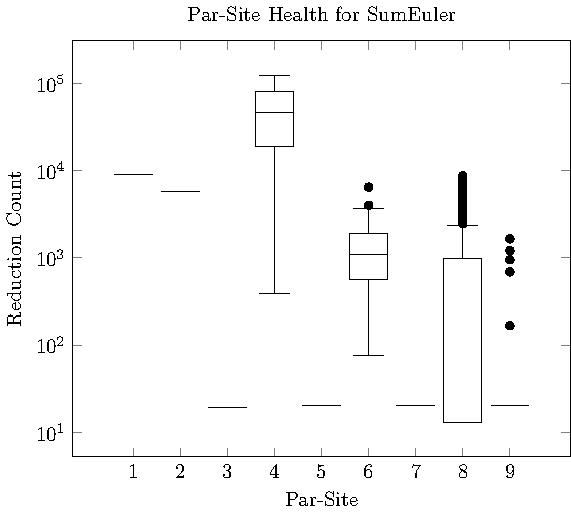
\includegraphics[width=\linewidth]{Informed/Figures/threadhealth.pdf}
\caption{Statistics on the number of reductions carried out by the threads a
\texttt{par} site sparks off}
\label{fig:sumHist}
\end{figure}

After every execution of the program, turn off the \verb'par' site whose threads
have the lowest average reduction count. In the case of the execution statistics
displayed in Figure \ref{fig:sumHist} we would disable \verb-par- site 2, allowing
us to avoid the overhead of all the unproductive threads it sparked off.  Then
repeat this process until switching a \verb'par' site off increases the overall
runtime of the program.

\section{Experimental Results}
\label{sec:results}

In this section we present some preliminary results and point out certain patterns
that appear in our data. 

First we introduce our benchmark programs and state the number of \verb-par-
sites that were introduced statically:

\subsection*{Overheads} Whether an expression is worthwhile to evaluate in
parallel is directly tied to \emph{cost} of creating a parallel task. In order
to account for this we ran all of our experiments with the simulated overhead
cost at 3 settings. We chose the upper and lower bounds based on benchmarking parallel
functions using the Criterion library \citep{criterion}.


For each program we set our runtime system to simulate 4, 8, and 16 cores.
First, let us examine Figure \ref{table10} which displays the results of setting
the cost of task creation to 10 reductions.

\begin{figure}[ht]
\centering
  \begin{tabular}{ |l||c c|c c|c c| }
    \hline
    Program & \multicolumn{2}{c|}{4-core} & \multicolumn{2}{c|}{8-cores} & \multicolumn{2}{c|}{16-cores} \\
    \hline
            & Runs & Final     & Runs & Final      & Runs & Final \\
    \hline
    SumEuler  & 6    & 3.77      & 6    & 6.84       & 6    & 10.27     \\
    Queens    & 5    & 1.30      & 5    & 1.37       & 5    & 1.41  \\
    Queens2   & 22   & 3.91      & 22   & 7.74       & 22   & 15.07   \\
    SodaCount & 3    & 2.42      & 3    & 4.72       & 3    & 8.95    \\
    Tak       & 1    & 3.39      & 1    & 6.79       & 1    & 13.58   \\
    Taut      & 4    & 1.00      & 0    & 1.00       & 9    & 1.00  \\
    MatMul    & 2    & 1.02      & 2    & 1.07       & 2    & 1.10   \\
    \hline
  \end{tabular}
\caption{Speedups relative to sequential computation when the cost of sparking
        a task is set to 10 reductions. The number of runs corresponds to the
        number of \texttt{par} sites that have been switched off.}
\label{table10}
\end{figure}

Already there are a few interesting results. \texttt{SumEuler} performs as expected and
manages to eliminate the majority of the introduced \verb-par- sites. Recalling
Figure \ref{sumLast}, the \verb-par-s that survive the iterative improvement
are the two in the \verb-main- function and the \verb-par- in \verb-mainListS2-.
The second \verb-par- in \verb-main- and the strategy \verb-mainListS2- are,
taken together, equivalent to applying \verb-parMap euler- over the input list.
When this program is parallelised explicitly, that \verb-parMap- is usually the
only addition to the program \citep{vGMachine}. It is reassuring that our
technique converges on the same result.

The two implementations of nQueens vary drastically in their improvement, with
the more symbolic solution (\texttt{Queens2}) achieving much better results. Search
problems are known to be problematic for techniques involving strictness
analysis and usually benefit from the introduction of \emph{speculative}
parallelism \citep{hammond2000research}.

\texttt{Taut} was chosen as a benchmark program specifically because the program (as
written) did not have many opportunities for parallelism. Had our technique
managed to find any useful parallelism, we would have been surprised.

MatMul is, to us, the most surprising of the results so far. Matrix
multiplication is famously parallelisable and yet our implementation
barely breaks even! Notice that of the 7 \verb-par- sites in MatMul, only
2 are being switched off. The \verb-par- setting that the iterative
improvement converged on was not the optimal setting (we know there is at least
2 superior settings). This convergence on local maxima is something we will
discuss in \S\ref{sec:conclusion}.

While the results in Figure \ref{table10} are revealing, it could be argued that
an overhead of 10 reductions to spark off a thread is unrealistically low.
Therefore we repeat the experiments with the more realistic 100 reduction
overhead (Figure \ref{table100}) and the pessimistic case of 1000 reduction
overheads (Figure \ref{table1000}).

\begin{figure}[ht]
\centering
  \begin{tabular}{ |l||c c|c c|c c| }
    \hline
    Program & \multicolumn{2}{c|}{4-core} & \multicolumn{2}{c|}{8-cores} & \multicolumn{2}{c|}{16-cores} \\
    \hline
            & Runs & Final     & Runs & Final      & Runs & Final \\
    \hline
    SumEuler  & 6    & 3.74      & 6    & 6.81       & 6    & 10.23     \\
    Queens    & 5    & 1.29      & 5    & 1.37       & 5    & 1.41  \\
    Queens2   & 22   & 3.83      & 22   & 7.57       & 22   & 14.76  \\
    SodaCount & 3    & 2.17      & 3    & 4.23       & 3    & 8.02    \\
    Tak       & 1    & 2.36      & 1    & 4.71       & 1    & 9.42   \\
    Taut      & 9    & 1.00      & 0    & 1.00       & 9    & 1.00  \\
    MatMul    & 2    & 0.93      & 2    & 1.06       & 2    & 1.09   \\
    \hline
  \end{tabular}
\caption{Speedups relative to sequential computation when the cost of sparking
        a task is set to 100 reductions. The number of runs corresponds to the
        number of \texttt{par} sites that have been switched off.}
\label{table100}
\end{figure}

The results in Figure \ref{table100} mostly align with what we would expect to
happen if creating a parallel task incurred higher overheads: we see reduced
speedup factors and adding more cores is less likely to benefit.

The key point to take away from this set of results is that while lower speedups
are achieved, the \emph{same} \verb-par- sites are eliminated in the same
number of iterations \footnote{Except for \texttt{Taut}, which in the 4-core case now
takes 9 runs to determine that there is no parallelism in the program.}.

Now we try the same experiment again but with the less realistic 1000 reduction
overhead to create a new thread.

\begin{figure}[ht]
\centering
  \begin{tabular}{ |l||c c|c c|c c| }
    \hline
    Program & \multicolumn{2}{c|}{4-core} & \multicolumn{2}{c|}{8-cores} & \multicolumn{2}{c|}{16-cores} \\
    \hline
            & Runs & Final     & Runs & Final      & Runs & Final \\
    \hline
    SumEuler  & 6    & 3.51      & 6    & 6.40       & 6    & 9.73     \\
    Queens    & 5    & 1.26      & 5    & 1.35       & 5    & 1.40  \\
    Queens2   & 22   & 3.14      & 22   & 6.22       & 22   & 12.18  \\
    SodaCount & 12   & 1.85      & 3    & 2.08       & 1    & 1.39    \\
    Tak       & 1    & 0.57      & 1    & 1.15       & 1    & 2.32   \\
    Taut      & 12   & 1.00      & 12   & 1.00       & 7    & 1.00  \\
    MatMul    & 5    & 1.00      & 5    & 1.00       & 5    & 1.01   \\
    \hline
  \end{tabular}
\caption{Speedups relative to sequential computation when the cost of sparking
        a task is set to 1000 reductions. The number of runs corresponds to the
        number of \texttt{par} sites that have been switched off.}
\label{table1000}
\end{figure}

While the speedups are now much more moderate (when there is a speedup at all)
these results are interesting for a few reasons.

In particular, the number of cores now has a greater influence on how many
\verb-par- sites are worthwhile.  \texttt{SodaCount}, for instance, now eliminates 12 of
its 15 \verb-par- annotations in the case of 4-core execution. This fits with
our intuition that when there are fewer processing units the threads require
coarser granularity to be worthwhile. In the cases of 8 and 16-core executions
we observe that fewer \verb-par- sites are disabled, reinforcing this
intuition.

MatMul also sees a jump in the number of disabled \verb-par- sites. Sadly, this
results in even worse performance for MatMul, which should be a highly
parallelisable program.

\subsection*{Static vs. Iterative}

While the results presented in Informed/Figures \ref{table10}, \ref{table100}, and
\ref{table1000} are promising for preliminary results they are based on an
admittedly simple search heuristic. Part of our argument is that static analysis
\emph{alone} is not sufficient for good gains from implicit parallelism. Figure
\ref{fig:iters} presents a selection of results that show how the iterative
improvement affects the static placement of \verb-par- annotations.

Even in the cases where the final speedup is lower than anticipated, such as
\texttt{Queens} in Figure \ref{fig:iterQueens}, the program still benefits from the
iterative improvement. \texttt{Queens2} sees the highest payoff from iterative
improvement. Many of the \verb-par-s introduced by the static analysis
do not contribute significantly to the computation even though it is
semantically safe to introduce them. The iterative loop converges on the few
\verb-par- sites that make a significant difference.

\begin{figure}[h]
    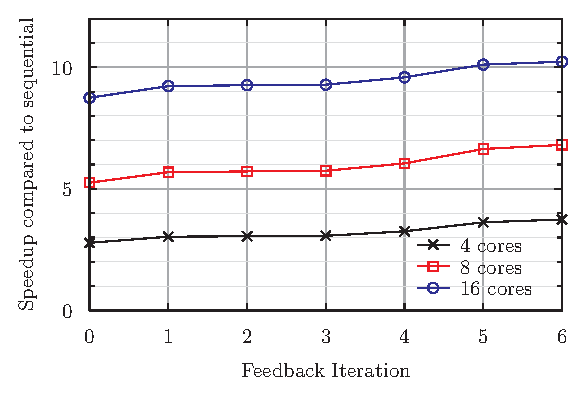
\includegraphics[scale=0.75]{Informed/Figures/IterSum.eps}
    \caption[SE]{\texttt{SumEuler} speedup}
    \label{fig:iterSum}
\end{figure}
\begin{figure}[h]
    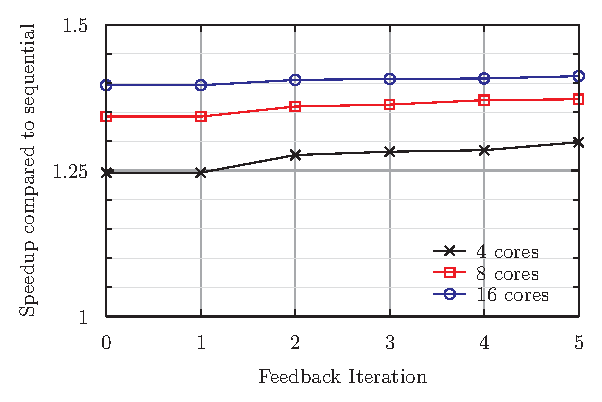
\includegraphics[scale=0.75]{Informed/Figures/IterQueens.eps}
    \caption[Q]{\texttt{Queens} speedup}
    \label{fig:iterQueens}
\end{figure}

\begin{figure}[h]
    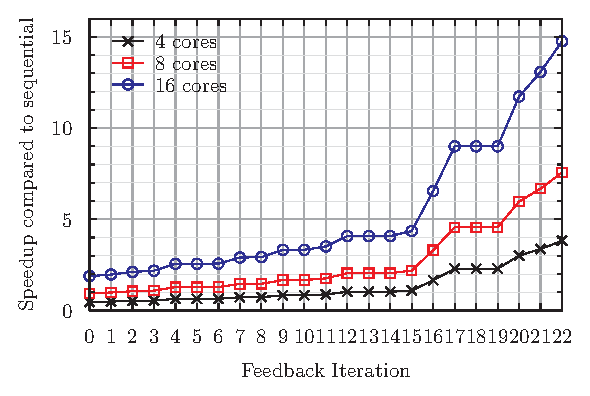
\includegraphics[scale=0.75]{Informed/Figures/IterQueens2.eps}
    \caption[Q2]{\texttt{Queens2} speedup}
    \label{fig:iterQueens2}
\end{figure}
\begin{figure}[h]
    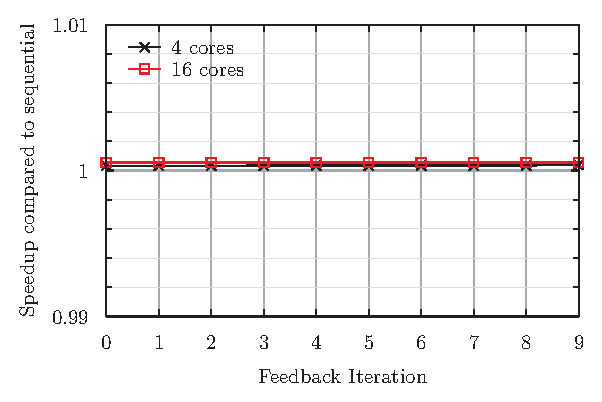
\includegraphics[scale=0.75]{Informed/Figures/IterTaut.eps}
    \caption[T]{\texttt{Taut} speedup}
    \label{fig:iterTaut}
\end{figure}


\subsection*{Comparison to GHC}

While the results above are encouraging we would like to see how the resulting
programs perform when compiled by a modern high-performance Haskell compiler.
To do this we extract the final \verb-par- settings from each program and
translate that to Haskell suitable for compilation by GHC.

For the versions parallelised by hand we use the \verb-par- placements found
in the literature \citep{vGMachine, runciman1994profiling}.

\begin{figure}[ht]
\centering
  \begin{tabular}{ |l||c c| }
    \hline
    Program & \multicolumn{2}{c|}{4-core} \\
    \hline
            & Hand   & Auto         \\
    \hline
    SumEuler  & 3.32    & 3.31      \\
    Queens    & 1.76    & 0.97      \\
    Queens2   & 2.29    & 0.61     \\
    SodaCount & 1.25    & 0.64      \\
    Tak       & 1.77    & 1.64      \\
    MatMul    & 1.75    & 0.80      \\
    \hline
  \end{tabular}
\caption{Speedups compared to the sequential program as compiled by GHC for both
         manually and automatically parallelised versions}
\label{tableGHC}
\end{figure}

As Table \ref{tableGHC} makes clear, the results are not impressive. In fact,
except for \verb-SumEuler- and \verb-Tak-, all of the parallel benchmarks
performed \emph{worse} than their sequential counterparts.

However, we feel that not all hope is lost. There are a few recurring issues in
the generated program. A common issue is that the generated strategies will not
be what forces the evaluation of a value. Take the following example as an
illustration

\begin{verbatim}
foo n = let ys = gen n n
        in par (tailStrict1 ys) (bar ys)

tailStrict1 xs = case xs of
    y:ys -> tailStrict1 ys
    []   -> ()
\end{verbatim}

In the function \verb-foo- we spark off a strategy that is meant to force the
spine of the list \verb-ys-, the catch is that GHC's \verb-par- is fast enough
for \verb-bar ys- to be what forces the evaluation of \verb-ys-. So we're
paying the overhead and reaping none of the benefits. In some programs changing
a \verb-par- like the one found in \verb-foo- to a \verb-seq- is enough to solve the
issue and make the parallel version competitive with the manually parallelised version.



\section{Conclusions}
\label{sec:conclusion}


We hope we have motivated the key design choices and ideas behind our compiler:
utilising defunctionalisation in \S\ref{sec:defunct}, and the use of
projections over other strictness analysis methods in \S\ref{sec:strictness}.
Moreover, that we have shown that there is a natural correspondence between
projections and strategies \S\ref{sec:proAndStrat} that allows us to generate
parallel strategies from the results of our strictness analysis.

While projection-based strictness analysis does provide a useful foundation for
the introduction of parallelism, the results in \S\ref{sec:results} show that
static analysis alone does not provide the desired speedups. Additionally,
Table \ref{tableGHC} shows that determining \verb-par--site health by reduction
count alone is too naive. Thread collisions that may not happen on a simulated
system are able to significantly hamper parallel performance and should be
taken into account.

\subsection{Related Work}

\subsection*{Hinze's Work on Projections} 

Much of the early work on strictness
analysis as a means to achieve implicit parallelism focused on the abstract
interpretation approach because the work on projections had not been fully
developed when implicit parallelism was a more active research area. In
particular, the work on the ``Automatic Parallelization of Lazy Functional
Programs'' \citep{hogen1992automatic} only used two and four-point domains (as
described in \citep{wadler1987strictness}) in their strictness analysis. This
limits the ability of the compiler to determine the neededness of more complex
structures.

Hinze's work on projection-based strictness analysis came after work on implicit
parallelism fell out of favour \citep{hinze1995projection, hammond2000research}. To
our knowledge we are the first to apply this work to the implicit parallelism.

\subsection{Comparison to Heuristic Search}

In the previous chapter we explored using two heuristic search algorithms to
accomplish our iterative step. While the results were promising, the ability to
examine profile data should not be underestimated. The first benefit is that
our search is guaranteed to be linear \emph{in the worst case} and usually
sub-linear, whereas even the greedy algorithm required exactly linear time.

As the programs grow larger the combinatorial explosion for the hill-climbing
will become more and more detrimental. For the hill-climbing algorithm to
terminate all neighbors to the current candidate must be explored. This means
that when a program has twenty \verb|par| sites, the \emph{last} iteration of
the hill-climbing algorithm will require twenty evaluations of the program! The
profile based technique's ability to guarantee that this program will require
\emph{at most} twenty iterations is a huge advantage.
